\section*{Sketch a line from its intercepts}

From Geometry, you know that 
you can draw a line through any two points.
You just connect the two points.
Maybe you use a ruler.
In particular, if you're given the $x$- and $y$-intercepts
of a line, sketch the line 
by getting out a ruler and drawing a line that passes 
through them both.

\begin{myConceptSteps}{To sketch the graph of a line from its intercepts\dots}
    \myStep{2-D grid}{Draw a 2-D $x$-$y$ grid.}
    \myStep{plot}{Plot the $x$-intercept as a dot on the $x$-axis.}
    \myStep{plot}{Plot the $y$-intercept as a dot on the $y$-axis.}
    \myStep{connect}{Connect the two dots with a straight line.}
\end{myConceptSteps}


\myBlankExample{2in}{
    Sketch the graph of the line with intercepts shown as big black dots on the graph below.
    \vskip1em
    \begin{center}
        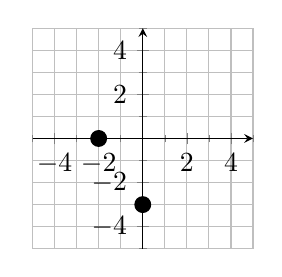
\begin{tikzpicture}
            \begin{axis}[
                width=2in,
                grid=both,
                axis x line = middle,axis y line = middle,
                axis equal image,
                xtick distance = 2, ytick distance = 2,
                xmin = -5, xmax = 5,
                ymin = -5, ymax = 5,
                minor tick num = 1,
                ]
                \addplot[
                    only marks,
                    mark=*,
                    mark size = 0.1cm,
                    ] coordinates { (0,-3) (-2,0) };
            \end{axis}
        \end{tikzpicture}
    \end{center}
}

\begin{taggedblock}{on-level}
    \myBlankExample{2.5in}{
        Sketch the graph of the line with 
        \begin{itemize}
            \item $x$-intercept at (3,0)
            \item $y$-intercept at (0,4)
        \end{itemize}
    }
\end{taggedblock}
\begin{taggedblock}{pre-AP}
    \myBlankExample{2.5in}{
        Sketch the graph of the line with 
        \begin{itemize}
            \item $x$-intercept at (-4,0)
            \item $y$-intercept at (0,-2)
        \end{itemize}
    }
\end{taggedblock}
